% !TeX root = ../main.tex

\chapter{基于时间序列异常检测的根因分析系统设计与实现}
\label{cha:root:cause:analysis}
\section{问题描述}
在复杂系统中,无论是微服务还是云网络的场景,一方面,会得到单点的多个指标数据,也就是单个点上多条时间指标序列,而且由于可能是不同类型的点(例如微服务中的操作系统、数据库、容器、中间件以及云网络中的网关、交换机、虚拟机、物理机等),其指标的模式以及指标的个数都不相同。另一方面,复杂系统中当出现异常时,异常会在系统中蔓延,在微服务中是通过服务调用的方式来传播,在云网络中则是流量收发包的方式。本文认为这种点与点之间的拓扑是已知的。当在一个给定时间点发生一个大规模异常时,有可能有多个节点以及多条链路发生故障,需要快速定位到是哪个节点最初发生故障并通过链路传播到了整个系统导致系统整体运行出现问题。

\section{框架设计}
本文设计的根因分析框架如图~\ref{fig:part2-overview}所示:
\begin{figure}[htbp]
    \centering
    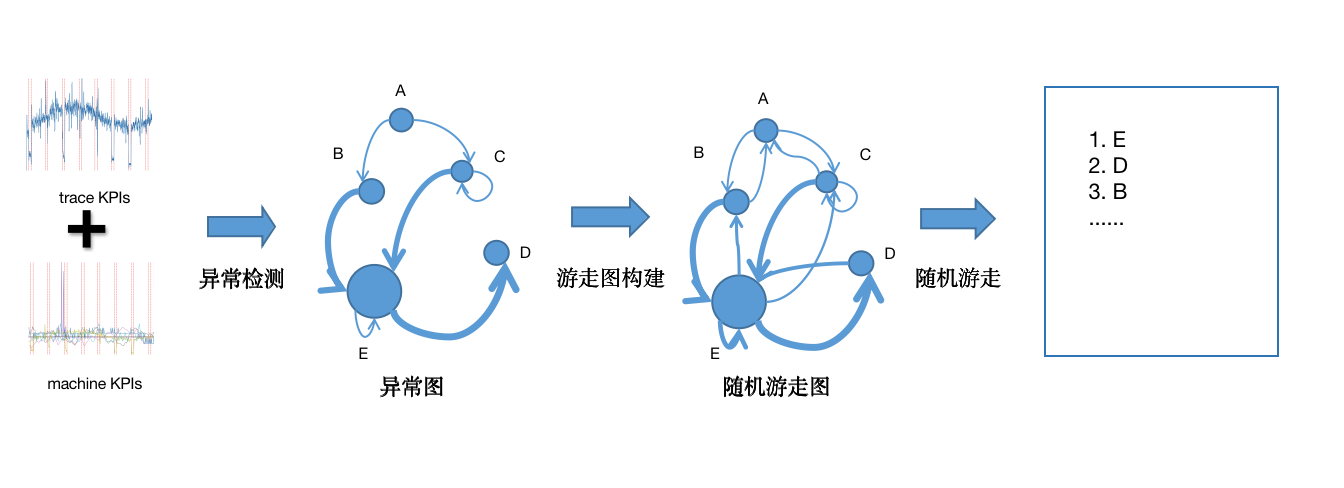
\includegraphics[width=\textwidth]{part2_overview.png}
    \caption{基于时间序列异常检测的根因分析系统框架}
    \label{fig:part2-overview}
  \end{figure}

首先通过预处理得到一系列节点上的时间序列数据和节点之间调用服务的相关指标(每分钟的调用次数、过去一分钟内的调用延时等)的时间序列数据,通过在故障时间点对这些时间序列数据运行异常检测算法得到这些曲线在该时刻的异常分数。用图的方式来可视化系统当前的状态:当一个节点的指标表现越异常,它的节点半径越大,如果一条边越异常,那么这条边就越粗。然后本文在这张图的基础上增加一些边以及修改一些边的权重,得到一张随机游走图。最后在图上运行随机游走算法来得到最有可能是根因的节点列表。接下来详细介绍各部分实现的细节。
\section{异常检测模块}
\label{sec:anomaly:detection}
在异常检测模块,需要在每个故障的时刻给出每个点以及每条边的异常程度。当数据量足够大的时候可以直接使用第~\ref{cha:anomaly:detection}章中使用的基于深度学习的方法,此处不再赘述;当数据量较小,例如每个点只有几百个采样点的时候,可以对每个单条的时间序列数据运用基于统计的方法得到一个异常分数,然后再用某个聚合函数(例如最大值或者平均值)将多个时间序列数据的分数变成单点/边的异常分数。

具体来讲,当数据点较少时,本文选择了KDE\footnote{Kernel Density Estimation,核密度估计}算法来做异常检测,因为其计算简单、通用性强,适用于各种特性的时间序列数据,基本思路是查看故障时间点后一段时间数据的分布与前一段时间数据分布的拟合情况,两者差别越大认为该数据异常程度越高。但实际使用中发现这个做法存在两个缺陷:一是会被偶然的尖刺影响到,而这种尖刺可能是统计错误或者其他原因造成的突发状况,但不足以构成异常;二是有明显长周期性的数据问题会影响到KDE算法的正确性,因为KDE只考虑了故障时间前后较短时间内的数据,因此如果有长周期特征的话,前后两个时间段的数据在分布上来看有很大的差别,但从长远上来看是符合历史特征的,这种不应该被判断为异常。因此本文选择在采用KDE算法之前去掉明显的尖刺,以及减去周期性的数据,消除这两部分的影响。另一方面,因为要将多个时间序列数据的异常分数进行聚合,而不同的时间序列数据可能具有不同的数量级,直接用KDE的话本身数据偏高的数据计算得到的异常分数也偏高。所以为了将所有异常分数放在一起比较,本文需要先将所有数据做归一化。因此,异常检测的步骤总结如下:第一步做归一化,第二步去掉尖刺数据,第三步进行周期性检测,将周期性数据从原数据中减掉,最后一步再进行KDE异常检测,输出一个异常分数。
\subsection{归一化}
目前常用的数据归一化方法主要是min-max和z-score标准化,考虑到min-max受异常值影响较大,本文采用了z-score标准化的方法。设原始数据的值为$x_i$,$mean$为原始数据的平均值,$std$为原始数据的标准差,则:
\begin{equation*}
y_i = \frac{x_i-mean}{std}
\end{equation*}

$y_i$为归一化后的数据,均值为0,方差为1,而且没有量纲。
\subsection{去除尖刺}
去除尖刺的目的是为了消除波动剧烈的数据对KDE算法带来的影响,该类尖刺往往持续时间较短,而且与前后的数据差别较大,因此本文针对做以下的平滑方式:
\begin{equation*}
z_i = \begin{cases} \frac{y_{i-1} + y_{i+1}}{2}, & y_i - y_{i-1} > th\ and\ y_i - y_{i+1} > th \cr \frac{y_{i-1} + y_{i+1}}{2} & y_{i-1} - y_i > th\ and\ y_{i+1} - y_i > th \cr y_i, & otherwise  \end{cases}
\end{equation*}

$z_i$则为去除尖刺后的数据。
图~\ref{fig:smooth}展示了一个去除尖刺的结果示例,其中两条红色虚线之间的是系统整体出现故障的区间。图~\ref{fig:smooth:left}显示,该数据仅在0:40-0:45呈现出较长时间的、与整体故障时间吻合的故障,而其他位置的尖刺则会影响到计算KDE分布时正常数据的分布,导致异常分数偏高,出现误报。从图~\ref{fig:smooth:right}中可以看出本文的处理方式很好地保留了真正的故障时段的异常,同时去除了其他时刻的尖刺,保证其他时刻不会被误报。

\begin{figure}[htbp]
  \begin{subfigure}[b]{0.5\textwidth}
    \begin{minipage}[t]{\linewidth}
    \centering
    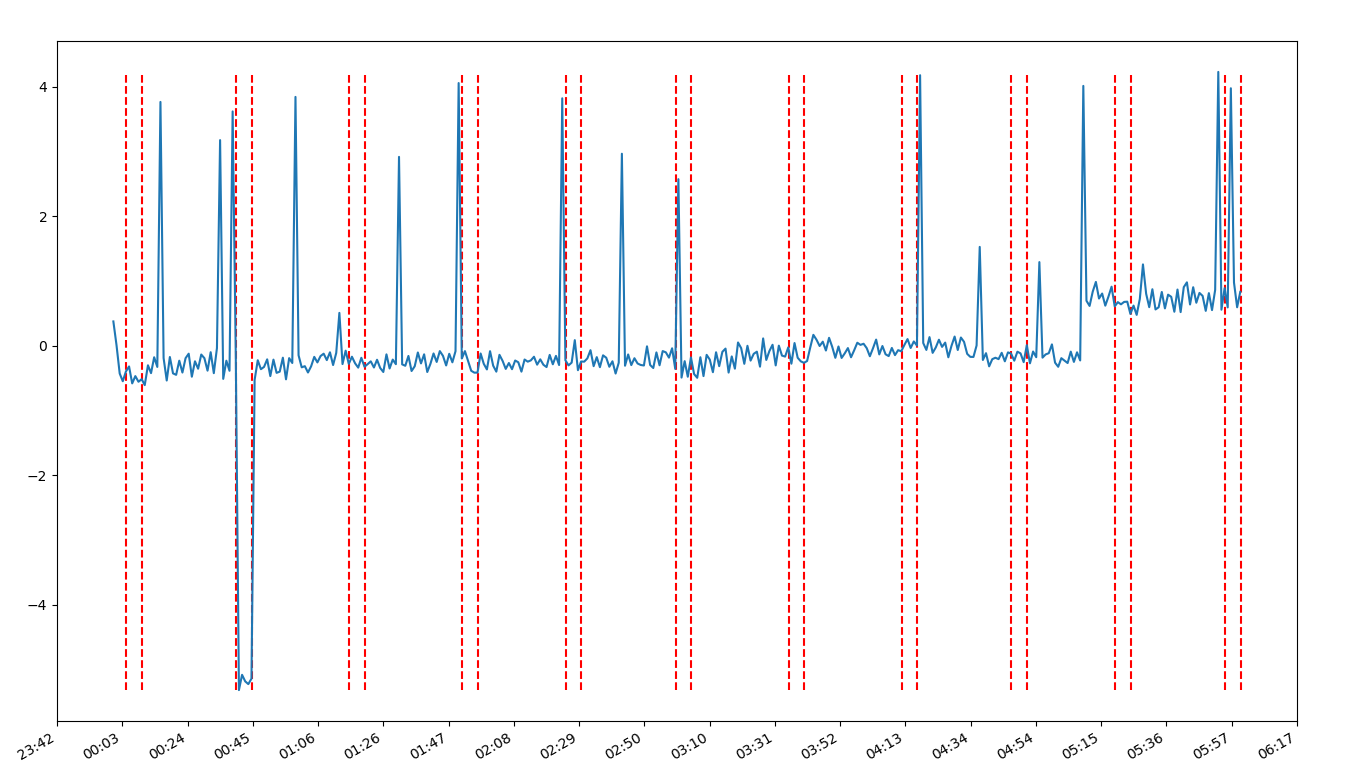
\includegraphics[width=\textwidth]{before_jian.png}
    \caption{原始数据}
    \label{fig:smooth:left}
    \end{minipage}
  \end{subfigure}
  \begin{subfigure}[b]{0.5\textwidth}
    \begin{minipage}[t]{\linewidth}
    \centering
    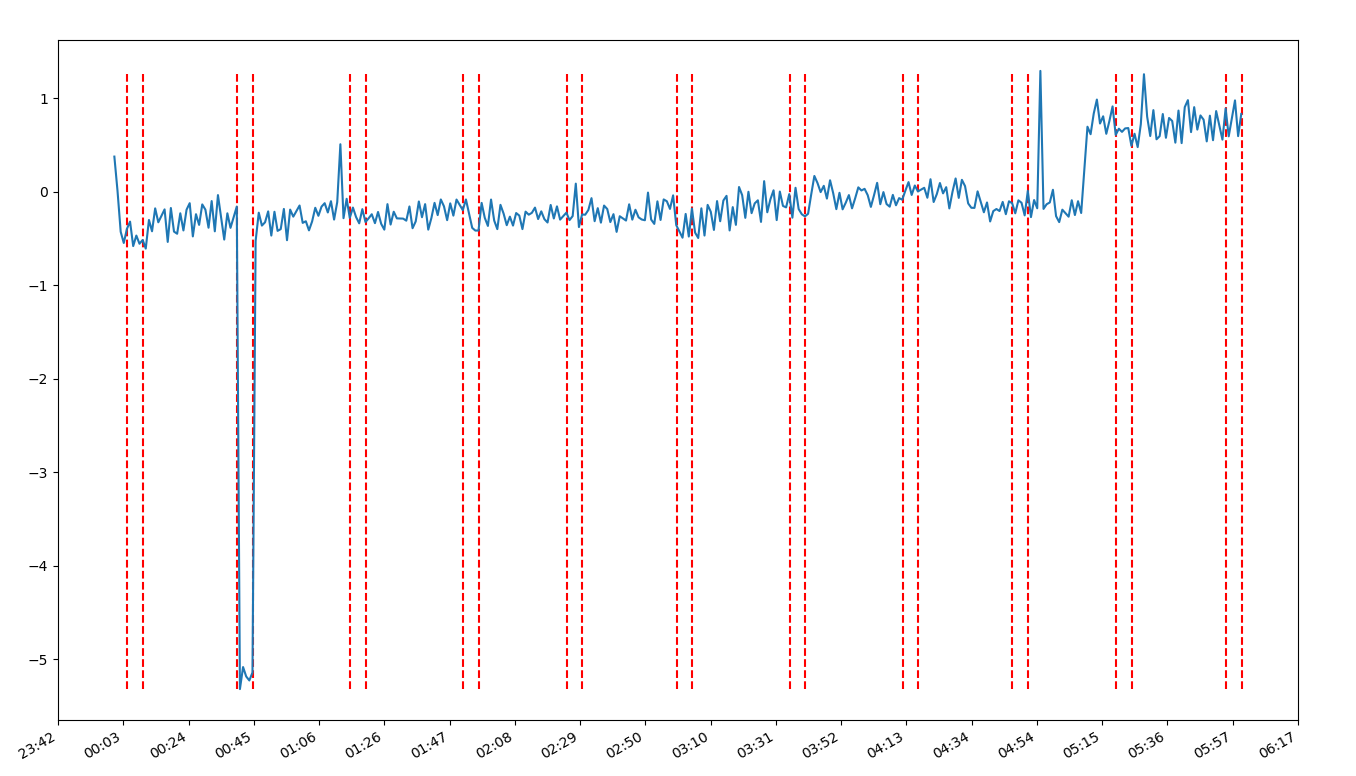
\includegraphics[width=\textwidth]{after_jian.png}
    \caption{去除尖刺后数据}
    \label{fig:smooth:right}
    \end{minipage}
  \end{subfigure}
    \caption{去除尖刺示例}
    \label{fig:smooth}
\end{figure}

\subsection{周期性数据去除}


在实际的时间序列数据中经常会遇到如图~\ref{fig:period:left}所示的数据,具有很强的周期性,这样的数据是符合历史特征的,所以不应该被判断为异常。但如果用KDE算法的话,只会考虑当前时间段与最近时间段的数据分布是否相似,不会考虑到较长时间之前的数据,所以要想让KDE算法仍然能够正常工作,需要将周期性也考虑进来。本文的思路是计算得到数据的周期,然后计算出每个周期每个位置的平均值,用原数据减去所在周期位置的平均值,之后再运行KDE算法,这样就考虑了周期性的影响。
\begin{figure}[htbp]
  \begin{subfigure}[b]{0.335\textwidth}
    \begin{minipage}[t]{\linewidth}
    \centering
    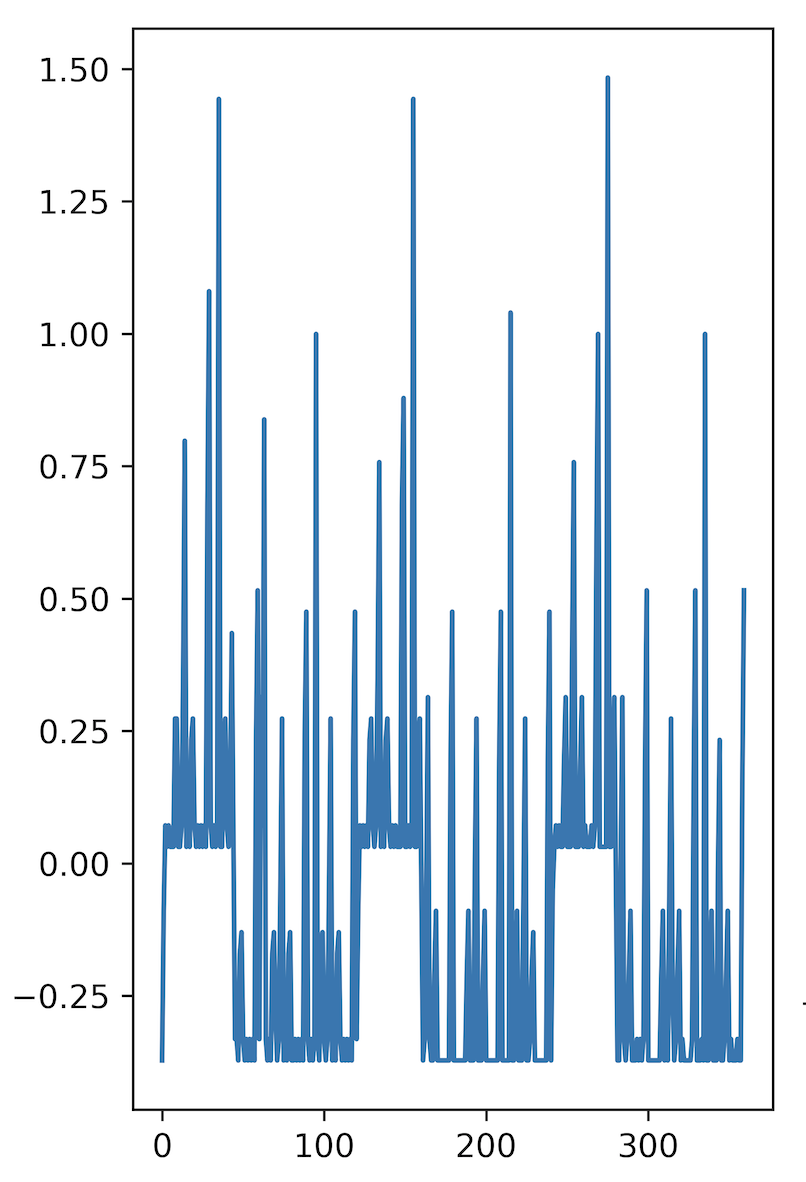
\includegraphics[width=\textwidth]{period_example_l.png}
    \caption{原始数据}
    \label{fig:period:left}
    \end{minipage}
  \end{subfigure}
  \begin{subfigure}[b]{0.325\textwidth}
    \begin{minipage}[t]{\linewidth}
    \centering
    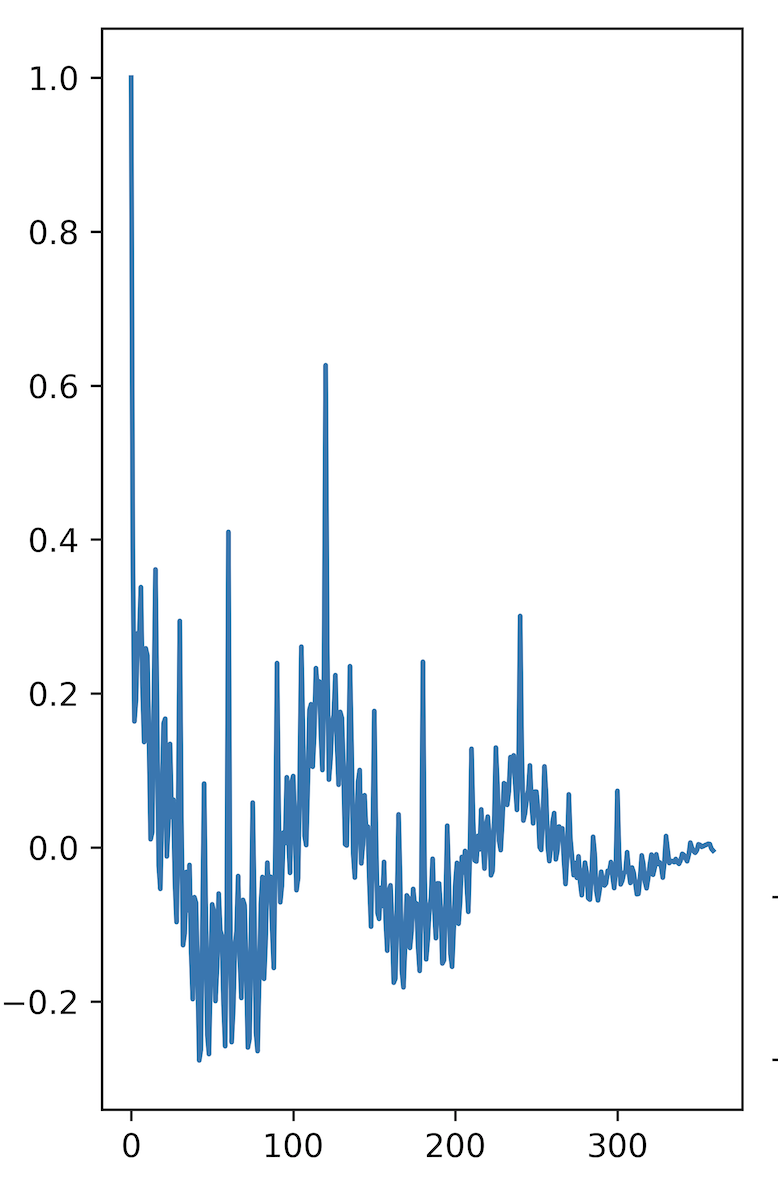
\includegraphics[width=\textwidth]{period_example_m.png}
    \caption{自相关函数}
    \label{fig:period:middle}
    \end{minipage}
  \end{subfigure}
  \begin{subfigure}[b]{0.325\textwidth}
    \begin{minipage}[t]{\linewidth}
      \centering
      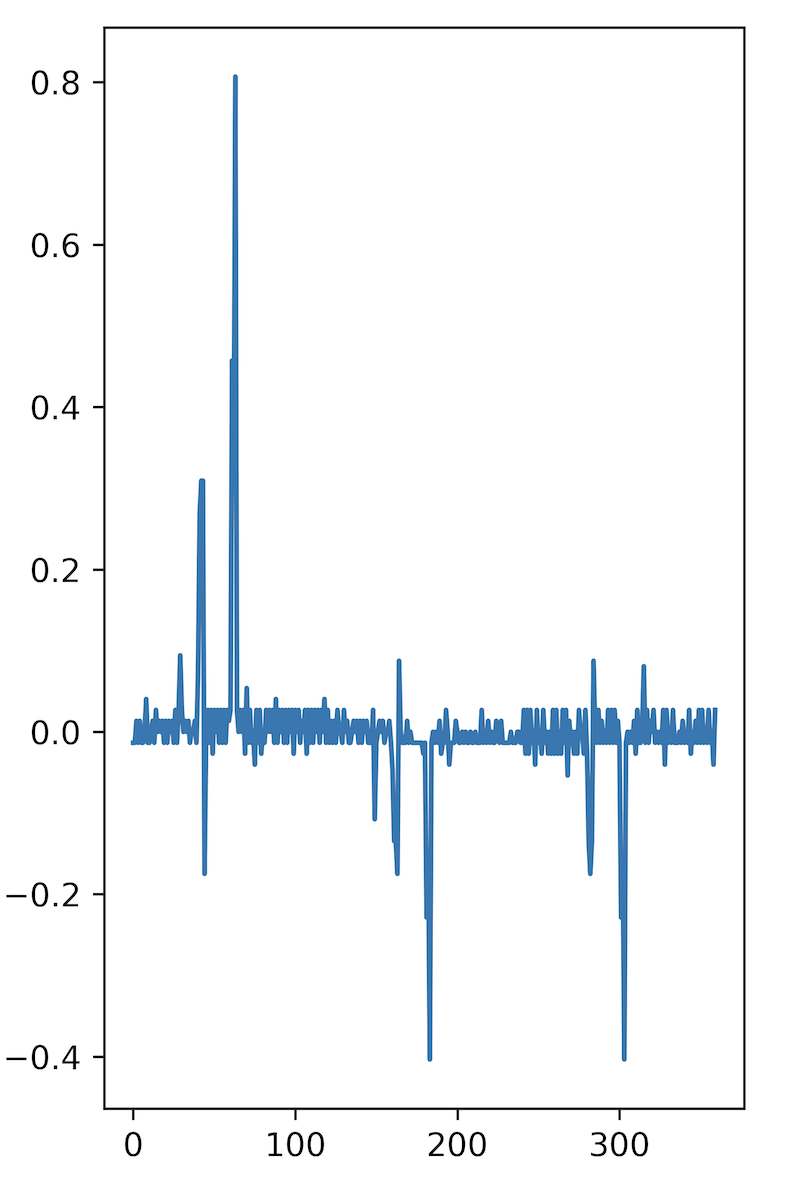
\includegraphics[width=\textwidth]{period_example_r.png}
      \caption{去除周期后的数据}
      \label{fig:period:right}
      \end{minipage}
    \end{subfigure}
    \caption{对数据去除周期化的过程}
    \label{fig:period}
\end{figure}

本文用自相关函数的方法来提取时间序列数据的周期\cite{rabiner1977use},自相关函数的计算方式为:
\begin{equation*}
  acf_i = \sum_{j=1}^{N-i}z_j\times z_{j+i}
\end{equation*}

从自相关函数的计算方式可以看出当$i$是数据的最小正周期的倍数的时候,函数值达到最大值。因此,在不考虑起始位置$i=0$的情况下,可以认为自相关函数的第一个最大值的位置就是数据的最小正周期$T$。从图~\ref{fig:period:middle}上可以确立出该数据的最小正周期为120。接下来再统计出周期内每个位置的平均数据,并且用原数据的每个位置减去他们在周期中所处位置平均值。即:

\begin{equation*}
  \begin{aligned}
  m_i = \frac{\sum_{j\%T = i}z_j}{\sum_{j\%T = i}1}\\
  w_i = z_i - m_{i\%T}
  \end{aligned}
\end{equation*}

将周期性数据减去之后得到处理好的数据如图~\ref{fig:period:right}所示,可以看到处理前的数据有大量的起伏,直接运行KDE算法会报出大量异常,而处理之后的数据尽管还留有少部分的尖刺(这是因为每两个尖峰之间的距离可能不能恰好的一个周期,因此在统计时没有完全对上),但大部分时间值的分布都在0附近,因此本文的方法能有效减少误报的数量。

\subsection{KDE异常检测}
KDE是概率论中用来估计未知函数密度的非参数检验的方法之一,可以根据观察到的样本来估计随机变量的概率密度函数。本文将一条时间序列数据近似看为一个随机变量的多个采样值,然后用KDE来估计概率密度函数。
\begin{equation*}
\hat{P}(w) = \frac{1}{n}\sum_{i=1}^nK(w;w_i)
\end{equation*}

其中$K$是可选取的核函数,$n$则是采样个数。KDE的核心思想就是对每个采样点形成一个一定带宽的核函数然后将所有采样点的核函数叠加起来作为对该数据的分布估计,当有了密度函数之后,就可以用来计算新出现的数据概率了。当给出故障时间点时,本文用前$T_a$时间内的数据来估计出一个密度函数,然后再来评估故障发生之后$T_b$时间内数据出现的概率,概率越低说明这段时间的数据越异常,那么异常分数就越高。设之后$T_b$时间内的数据为$w_1,w_2,\dots,w_k$,而前$T_a$时间内的数据用KDE估计得到的密度函数为$\hat{P}(w)$,则异常分数为:
\begin{equation*}
  Score = \frac{1}{k}\sum_{i=1}^k\ln P(w_i)
\end{equation*}

其中求均值是为了消除$T_b$时间内不同曲线可能采样点个数不同带来的影响。

得到了每条时间序列数据在该时刻的异常分数之后,需要将多条曲线的值聚合到点或者边上。对于一个点来说,本文认为它的异常分数就是所有异常分数的最大值,因为这些时间序列数据之间可能是不相关的,比方说某个时刻内只有发包数发生了异常其他指标都工作正常,也足以认为是出现了异常;而对于边来说,因为有重边的存在,本文认为边的异常分数是所有重边的异常分数的平均值,因为这些数据是相关的,都是表示从一个节点调用另一个节点的服务情况,如果出现异常的话,所有的曲线应该都有一个较高的异常分数,如果只有一条曲线的分数较高则有可能是异常检测算法不准导致的偶然情况。至此本文得到了一张异常图,来描绘当前系统中各点和各边的异常情况,如图~\ref{fig:part2-overview}异常图所示。
\section{根因分析模块}
这部分要在异常图的基础上构建出随机游走图,再通过随机游走得出经过每个点的次数,经过次数越多则越可能是根因。


\subsection{构建随机游走图}
不妨设~\ref{sec:anomaly:detection}节得到的异常图为$G=(V,E)$,点$i$的点权为$v_i$,边权为$w_{i,j}$。要构建的随机游走图由以下三种边组成:
\begin{itemize}
  \item 前向边:为了运行随机游走算法,边的方向应当代表异常传播的方向。当一个$i$调用$j$的服务调用时长发生异常时,本文认为异常是由$j$传播到$i$,因此异常传播的方向与服务调用的方向相反,也就是根因的方向与服务调用的方向相同。所以该部分保持不变;
  \item 反向边:因为随机游走具有一定的随机性,为了防止行走者走到一个较小概率是根因的节点,然后出不去,本文考虑加入反向边。该边的权值随正向边的权值增加而增加,也就是$w_{i,j} = \rho_{back} w_{j,i}$,如果$(i,j) \notin E\ and\  (j,i) \in E$;
  \item 自环:当节点自身就是根因的时候,需要增大其留在原位置的概率而不走到其他地方。本文观察到:当一个节点是根因时,它会影响到周围和它有关联的点,通常情况下所有调用它的服务的返回时间都会出现异常,同时它调用其他节点的服务也会出现异常,因此本文要将这些因素也纳入考量范围。总的来说需要考虑三个因素,一是节点本身的异常分数,二是所有其他节点到该节点的边的异常分数的平均值,三是该节点到所有其他节点的边的异常分数的平均值,也就是$w_{i,i} = \rho_{in} in\_avg\_weight_{i} + \rho_{out} out\_avg\_weight_{j}+ \rho_{self}  v_i$。另一方面,考虑到入边是推导根因的方向,所以本文在设置超参时会保证$\rho_{in}>\rho_{out}$。
\end{itemize}

总结如下:
\begin{equation*}
w_{i,j} = \begin{cases} w_{i,j}, & if\ (i,j) \in E \cr \rho_{back} w_{j,i}, &\ if\ (i,j) \notin E\ and\  (j,i) \in E \cr \rho_{in} in\_avg\_weight_{i} + \rho_{out} out\_avg\_weight_{j}+ \rho_{self}  v_i, & if\ i=j \end{cases}
\end{equation*}

\subsection{随机游走}
首先将边权矩阵$w$标准化得到转移矩阵$\overline{w}$:
\begin{equation*}
  \overline{w}_{i,j} = \frac{w_{i,j}}{\sum_jw_{i,j}}
\end{equation*}

然后在整张图中随机起点开始行走,当处于位置$i$时,有$p$的概率随机到达图中任一位置,有$1-p$的概率沿图中的边行走,而到达相邻点$j$的概率就为$(1-p)\overline{w}_{i,j}$,行走一定的次数之后,统计每个点被经过的次数$R_i$,经过次数越多的则越有可能是根因。随机游走过程如算法~\ref{algorithm:random:walk}所示。

\begin{algorithm}
  \caption{随机游走过程}
  \begin{algorithmic}[1]
      \Require $p,V,\overline{w},step$
      \Ensure $R$
      \State $v$ \gets randomly choose from $V$
      \Repeat
      \State $r \gets random(0,1)$
      \If {$r < p$}
        \State $v$ \gets randomly choose from $V$
      \Else
        \State $v$ \gets randomly choose $j$ by $\overline{w}_{v,j}$ probability
      \EndIf
      \State $R_i \gets R_i + 1 $
      \Until {$step$ rounds}
      \State sort $R$ in descending order
  \end{algorithmic}
  \label{algorithm:random:walk}
\end{algorithm}
\section{实验评估}
本文采用AIOPS2020挑战赛作为验证算法效果的数据集。

\subsection{数据集介绍}

该数据集是一个微服务场景下的复杂系统数据集,整个系统如图~\ref{fig:static_topo}所示。提供了所有节点包括操作系统、容器和数据库的指标以一定时间间隔采样得到的指标信息,并且还有不同节点之间调用服务的记录。实际测试中,会得到若干个时间段,表示在这个时间段上整个系统出现了问题。需要找出的根因分为网络故障和节点故障,节点故障需要给出某个节点的某个指标,而网络故障如果在主机上需要给出指标,否则只需要定位到节点即可。具体的故障信息如表~\ref{tab:error}所示。

\begin{figure}[htbp]
    \centering
    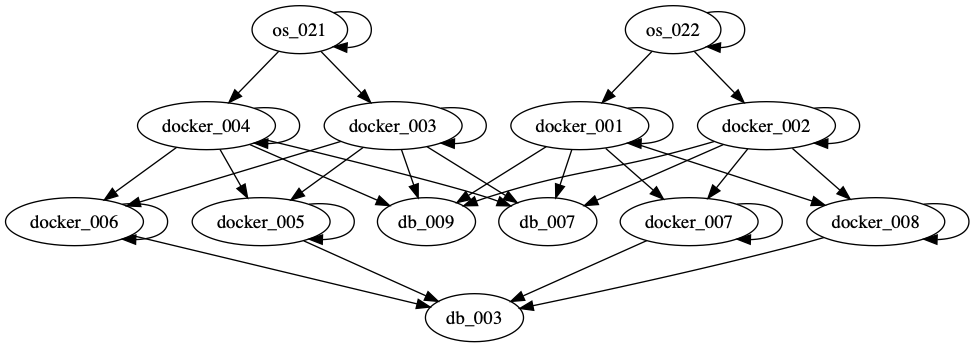
\includegraphics[width=\textwidth]{static_topo.png}
    \caption{静态拓扑图}
    \label{fig:static_topo}
  \end{figure}

\begin{table}[htbp]
  \centering
  \begin{tabular}{ccc}
    \toprule
    技术栈 & 场景名称 & 定位需求\\
    \midrule
    \multirow{2}{*}{数据库oracle} & 数据库关监听 & 节点指标\\
     & 数据库连接限制 & 节点指标 \\
    \multirow{3}{*}{DCOS容器} & CPU压测 & 节点指标\\
     & 网卡丢包 & 节点\\
     & 网卡延迟 & 节点\\
    \multirow{2}{*}{主机} & 网络丢包& 节点指标\\
    & 网络延迟 & 节点指标\\
    \bottomrule
  \end{tabular}
  \caption{根因类别}
  \label{tab:error}
\end{table}

\subsection{实验设置}
超参数的设置方面,KDE算法中本文采用了高斯核函数,带宽取0.4,选择故障前后时间窗口的部分因为该数据集的故障持续时间均为5分钟,故$T_a$设置为15分钟,$T_b$设置为5分钟;根因定位方面构图的超参根据经验依次设置$\rho_{back}=0.5, \rho_{in} = 0.6, \rho_{out} = 0.3, \rho_{self} = 0.5$,随机游走的$p$设置为$0.1$,$step$则设置为10000步。

在结果输出方面,有两个要特别注意的地方。一是在该数据集中,存在两个容器例如docker001和docker005位于同一个主机os017上而该主机不出现在拓扑图上的情况,如图~\ref{fig:two:rca}所示,docker001和docker005像两个独立的根因,这种情况下要定位到os017。本文的做法是选取随机游走经过次数前二的点,判断其是否均为容器且位于同一主机上,如果是则定位到它们所属的主机上;另一个则是该数据集要求定位到具体的指标,如果是网络异常则不用输出指标。通过观察发现,网络异常往往的表现就是本身指标没有过于异常的,所以本位在定位到节点之后找到异常分数最大的指标,如果其指标异常分数大于某个阈值认为它是根因,否则认为是网络故障。

\begin{figure}[htbp]
  \centering
  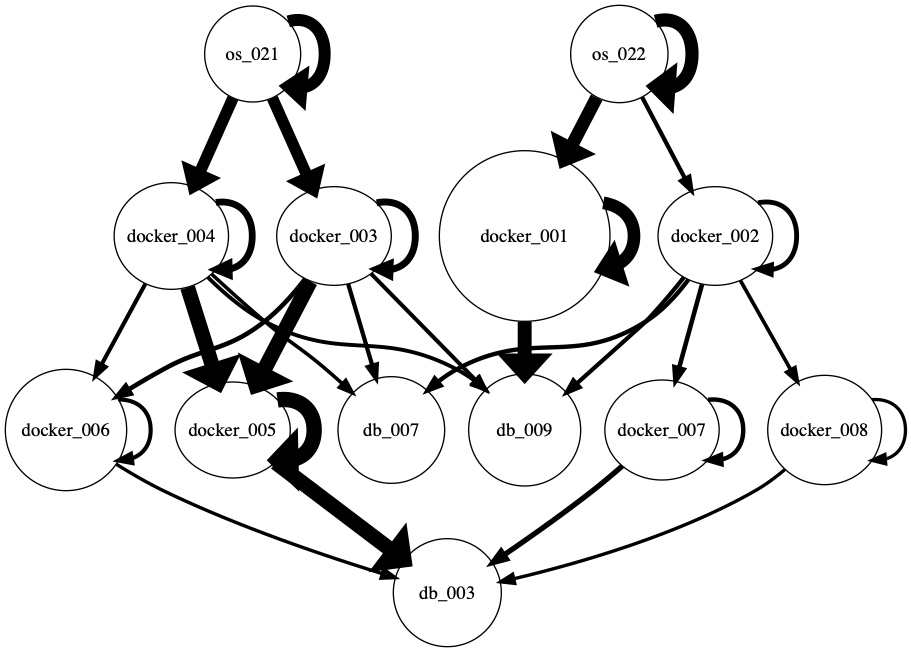
\includegraphics[width=0.8\textwidth]{two_rca.png}
  \caption{数据集中的一个特例}
  \label{fig:two:rca}
\end{figure}


\subsection{baseline选取}
本文选取的baseline为在异常检测之后根据自身的异常分数以及相连边的异常分数之和排序然后选取最高的作为根因,在结果输出时与本文的方法保持一致。
\subsection{实验结果分析}
该数据集一共有7批数据,分别有11、11、3、10、10、6和5个测试点,本文的方法与baseline的方法在各批数据的正确率如表~\ref{tab:rca:result}所示。

\begin{table}[htbp]
  \centering
  \begin{tabular}{ccccccccc}
    \toprule
      & 第一批 & 第二批 & 第三批 & 第四批 & 第五批 &第六批 & 第七批& 总体\\
    \midrule
    baseline & 0.64 & 0.73 & 1& 0.6 & 0.91 & 0.5 &0.5  & 0.69\\
    ours &  0.91 & 0.91 & 1 & 0.9 & 0.91 &1 & 0.83 & 0.91\\
    \bottomrule
  \end{tabular}
  \caption{根因定位准确率对比}
  \label{tab:rca:result}
\end{table}

从中可以看出,使用随机游走的方法比直接在异常图上进行统计的方法准确率高出二十个百分点。而本文的方法未能准确检测的三个根因中有两个是根因和所得到的静态拓扑图完全没有关系的,而另两个则如图~\ref{fig:bad:case}所示。真正的根因是docker001的网络故障,而本文的算法定位到了os022的网络故障上,docker001在经过次数中排名第三位。所以在这种影响范围较小的情况下本文的算法准确性会出一点问题。一些准确定位的故障其异常图如~\ref{fig:error:example}所示。当出现容器网络这一类故障例如图~\ref{fig:error:docker:network}时,baseline的方法则有可能会定位到os022,而随机游走则会避免这一错误,通过在图上不断地游走,最后经过正确答案docker007的次数最多,并且,当系统的规模扩大时,baseline针对单点的统计更有可能出错,因为当调用链的长度增加时,会出现多个节点的异常分数与边的异常分数之和极大的情况,而真正的根因则需要用随机游走的方式,通过模拟异常传播的方式才能从调用链上推断出来。
\begin{figure}[htbp]
  \centering
  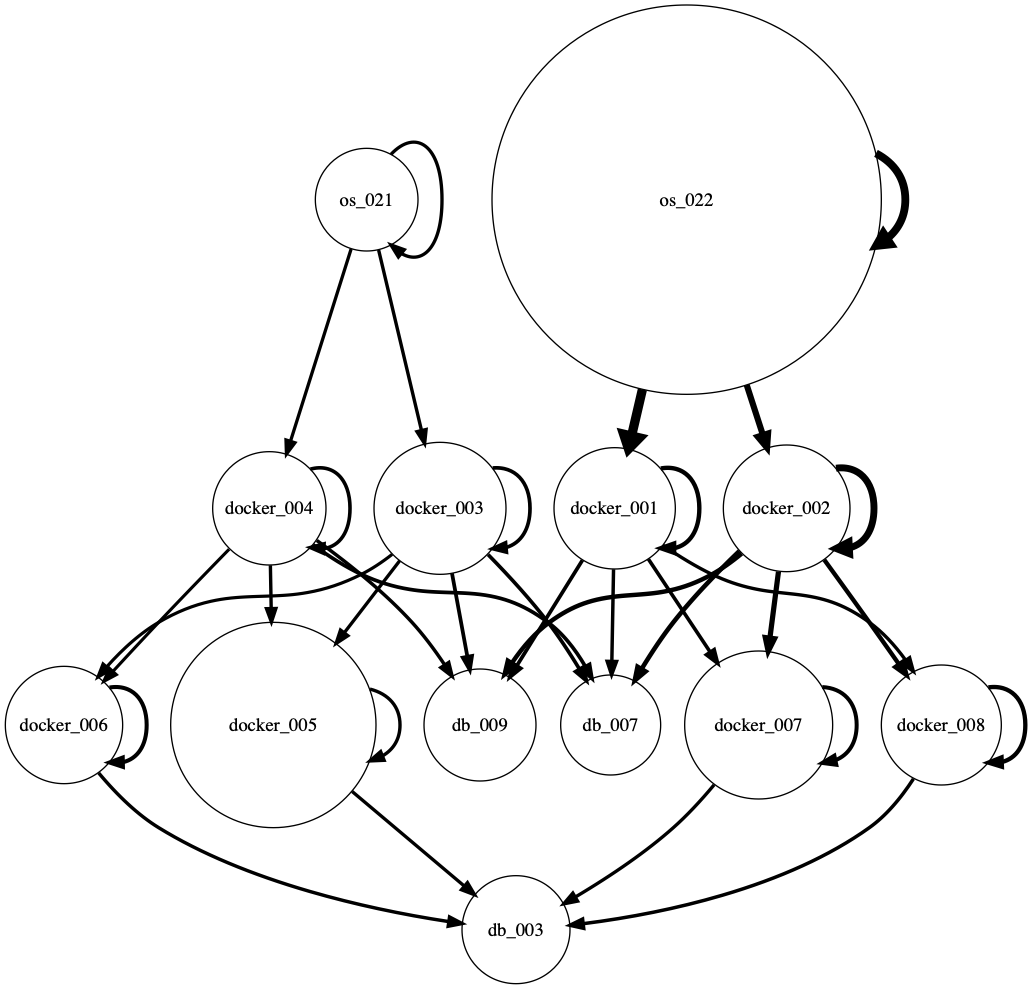
\includegraphics[width=0.8\textwidth]{bad_case.png}
  \caption{本文算法的一个bad case}
  \label{fig:bad:case}
\end{figure}

\begin{figure}[htbp]
  \centering
  \begin{subfigure}[b]{\textwidth}
    \begin{minipage}[t]{0.5\linewidth}
      \centering
      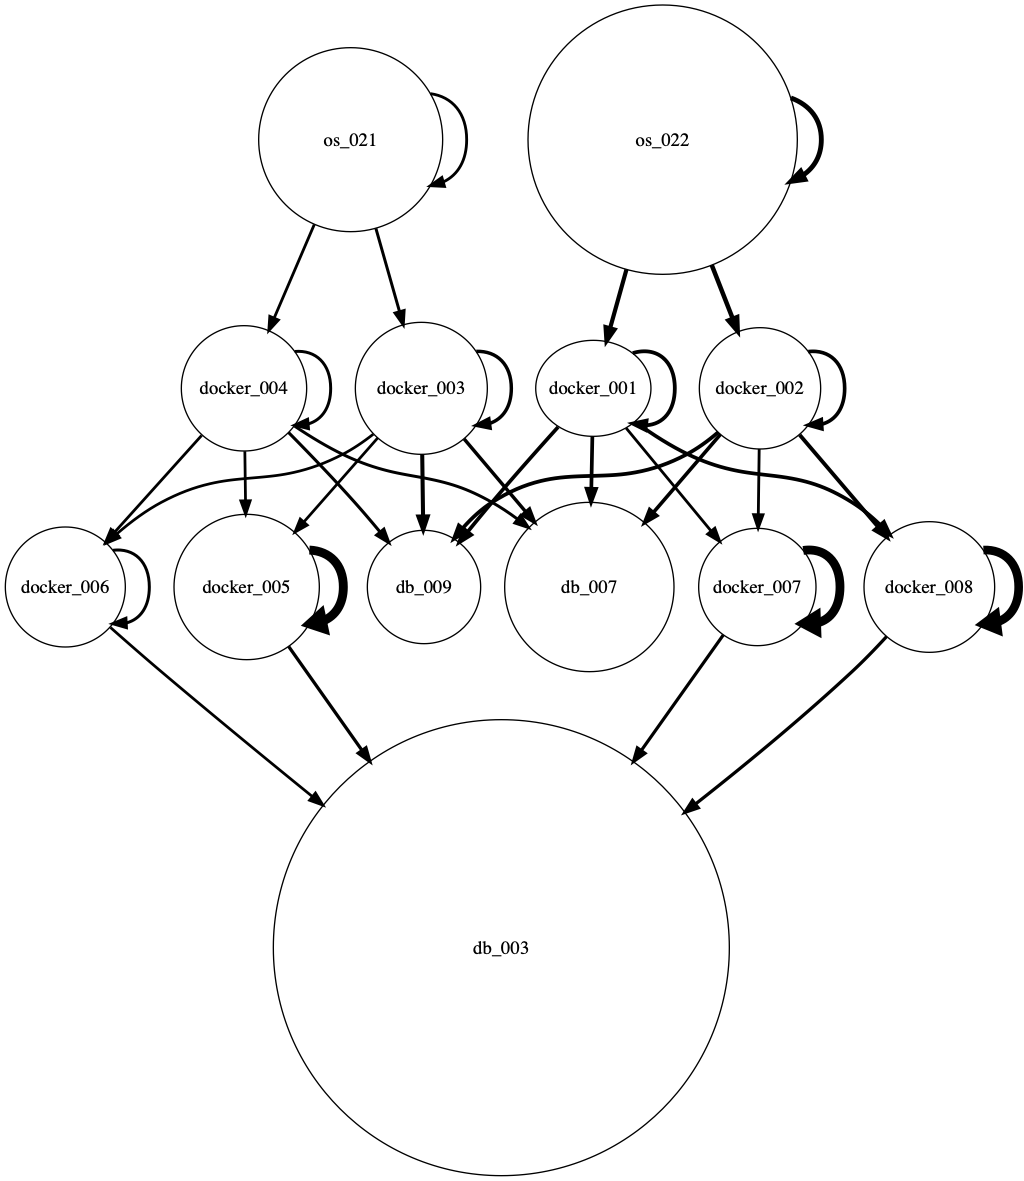
\includegraphics[width=\textwidth]{db_error.png}
      \caption{数据库关监听}
      \label{fig:error:db}
    \end{minipage}
    \begin{minipage}[t]{0.5\linewidth}
      \centering
      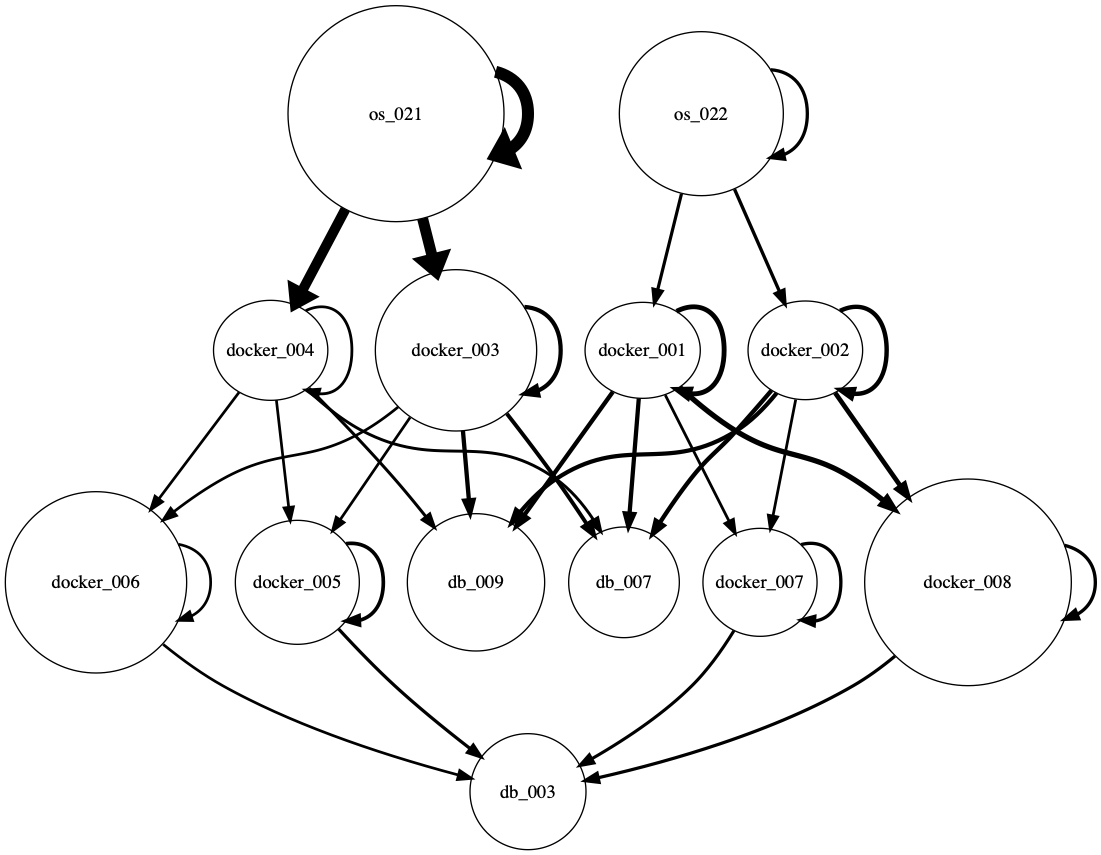
\includegraphics[width=\textwidth]{os_error.png}
      \caption{主机网络故障}
      \label{fig:error:os}
    \end{minipage}
  \end{subfigure}

  \begin{subfigure}[b]{\textwidth}
    \begin{minipage}[t]{0.5\linewidth}
      \centering
      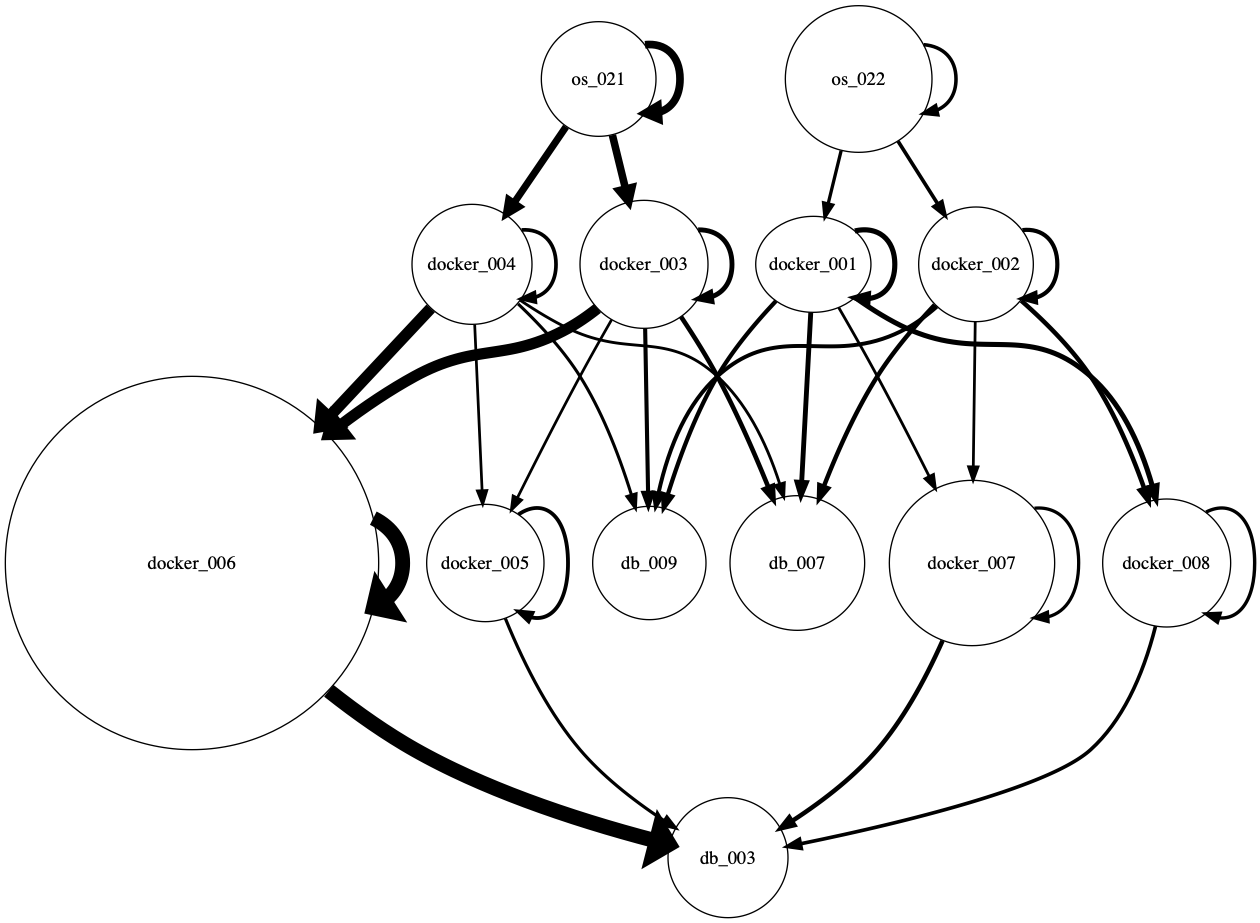
\includegraphics[width=\textwidth]{docker_cpu_error.png}
      \caption{容器cpu压测}
      \label{fig:error:docker}
    \end{minipage}
    \begin{minipage}[t]{0.5\linewidth}
      \centering
      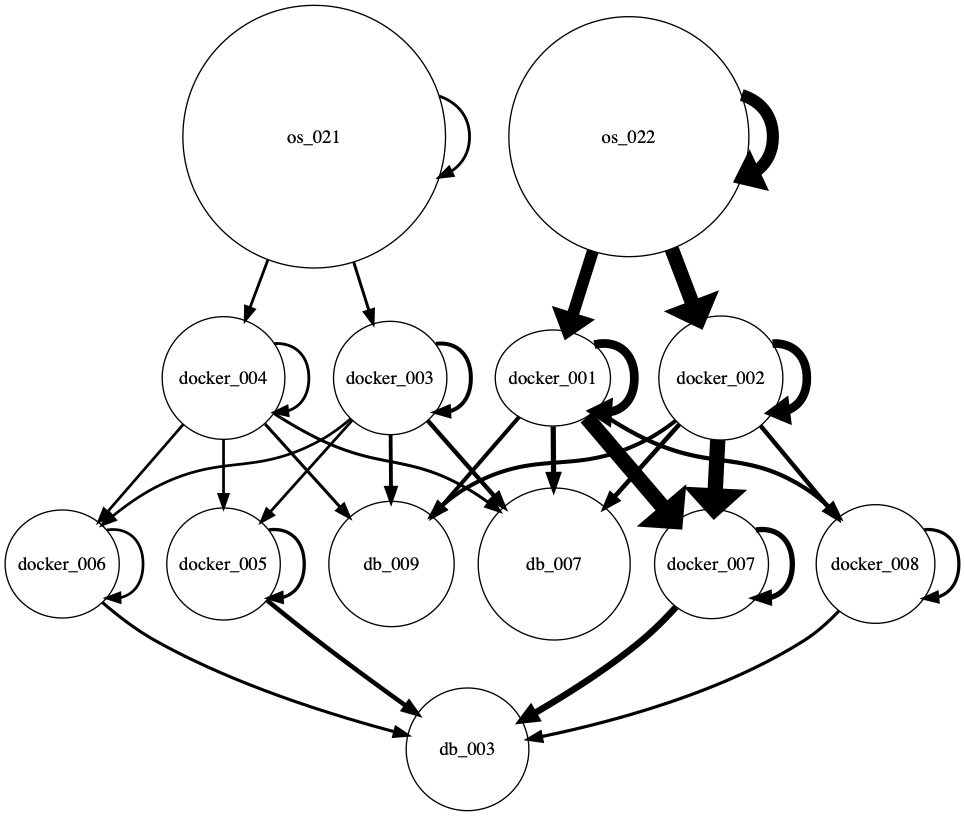
\includegraphics[width=\textwidth]{docker_network_error.png}
      \caption{容器网络故障}
      \label{fig:error:docker:network}
    \end{minipage}
  \end{subfigure}
  \caption{AIOPS2020挑战赛中故障示例}
  \label{fig:error:example}
\end{figure}

\section{小结}
本章详细介绍了基于时间序列异常检测的根因分析系统,对节点上的时间序列数据和节点之间的服务调用相关的时间序列数据运行KDE异常检测算法得到异常分数,以此为基础构建异常传播图,在这个图上进行随机游走算法来得到每个节点的经过次数,最多的即认为是根因。所用方法在AIOPS2020上验证得到了较高的准确率。